\documentclass[a4paper,12pt]{article}
\usepackage{color}
\usepackage{graphicx, gensymb}
\usepackage{amsfonts, cancel, amssymb}
\usepackage{amsmath, amsthm, array, esvect, esint}
\usepackage{typearea}
\usepackage[a4paper,left=2cm,right=2cm,top=2cm,bottom=3cm,bindingoffset=5mm]{geometry}
\usepackage{tikz} 
\usetikzlibrary{shapes,arrows,positioning,automata,backgrounds,calc,er,patterns}
\usepackage{tikz-feynman}
\tikzfeynmanset{compat=1.0.0}
\newcommand\numberthis{\addtocounter{equation}{1}\tag{\theequation}}
\newcommand{\bra}{}
\newcommand{\kom}{}
\newcommand{\brak}{}
\newcommand{\braket}{}
\newcommand{\intx}{}
\newcommand{\intr}{}
\newcommand{\kla}{}
\newcommand{\klam}{}
\newcommand{\klammer}{}
\newcommand{\oper}{}
\newcommand{\tecxt}{}
\newcommand{\Bra}{}
\newcommand{\Ket}{}

\begin{document}

\title{Feynman-Diagramme}
\author{Joachim Schwardt}
\date{\today}
\maketitle


\section*{Aufgabe 6.2: Feynman-Diagramme}
%\begin{tikzpicture}
%\begin{feynman}
%\vertex (a) {\(\mu^{-}\)};
%\vertex [right=of a] (b);
%\vertex [above right=of b] (f1) {\(\nu_{\mu}\)};
%\vertex [below right=of b] (c);
%\vertex [above right=of c] (f2) {\(\overline \nu_{e}\)};
%\vertex [below right=of c] (f3) {\(e^{-}\)};
%\diagram* {
%(a) -- [fermion] (b) -- [fermion] (f1),
%(b) -- [boson, edge label'=\(W^{-}\)] (c),
%(c) -- [anti fermion] (f2),
%(c) -- [fermion] (f3),
%};
%\end{feynman}
%\end{tikzpicture}
Für den Prozess $e^-e^+\longrightarrow e^-e^+$:
\begin{figure}[h!]
\centering
\begin{minipage}{0.4\textwidth}
\centering
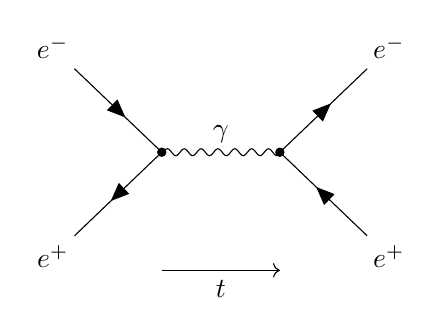
\begin{tikzpicture}
\begin{feynman}
\vertex (a);
\vertex [right=of a] (b);
\vertex [below=of a] (t1);
\vertex [below=of b] (t2);
\vertex [above left=of a] (f1){$e^-$};
\vertex [below left=of a] (f2){$e^+$};
\vertex [above right=of b] (f3){$e^-$};
\vertex [below right=of b] (f4){$e^+$};
\diagram*{
(f1) -- [fermion] (a) -- [fermion] (f2),
(a) -- [boson, edge label=$\gamma$] (b),
(f4) -- [fermion] (b) -- [fermion] (f3),
};
\end{feynman}
\draw[->] (t1) -- (t2) node[midway, below] {$t$};
\fill (a) circle (0.06cm);
\fill (b) circle (0.06cm);
\end{tikzpicture}
\caption{s-Kanal}
\end{minipage}
\begin{minipage}{0.4\textwidth}
\centering
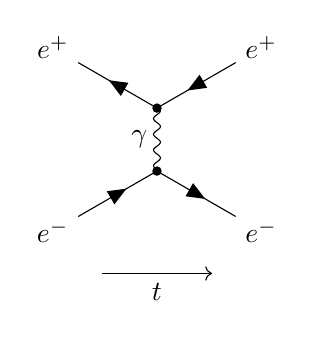
\begin{tikzpicture}
\begin{feynman}
\vertex (a);
\vertex [above=0.8cm of a] (b);
\vertex [below left=1.3cm and 0.7cm of a] (t1);
\vertex [below right=1.3cm and 0.7cm of a] (t2);
\vertex [below right=0.5cm and 1cm of a] (f1){$e^-$};
\vertex [below left=0.5cm and 1cm of a] (f2){$e^-$};
\vertex [above right=0.5cm and 1cm of b] (f3){$e^+$};
\vertex [above left=0.5cm and 1cm of b] (f4){$e^+$};
\diagram*{
(f2) -- [fermion] (a) -- [fermion] (f1),
(a) -- [boson, edge label=$\gamma$] (b),
(f3) -- [fermion] (b) -- [fermion] (f4),
};
\end{feynman}
\draw[->] (t1) -- (t2) node[midway, below] {$t$};
\fill (a) circle (0.06cm);
\fill (b) circle (0.06cm);
\end{tikzpicture}
\caption{t-Kanal}
\end{minipage}
\end{figure}\\
Für den Prozess $e^-\mu^+\longrightarrow e^-\mu^+$:
\begin{figure}[h!]
\centering
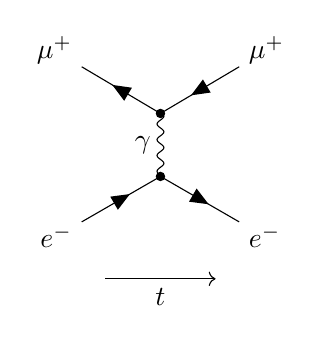
\begin{tikzpicture}
\begin{feynman}
\vertex (a);
\vertex [above=0.8cm of a] (b);
\vertex [below left=1.3cm and 0.7cm of a] (t1);
\vertex [below right=1.3cm and 0.7cm of a] (t2);
\vertex [below right=0.5cm and 1cm of a] (f1){$e^-$};
\vertex [below left=0.5cm and 1cm of a] (f2){$e^-$};
\vertex [above right=0.5cm and 1cm of b] (f3){$\mu^+$};
\vertex [above left=0.5cm and 1cm of b] (f4){$\mu^+$};
\diagram*{
(f2) -- [fermion] (a) -- [fermion] (f1),
(a) -- [boson, edge label=$\gamma$] (b),
(f3) -- [fermion] (b) -- [fermion] (f4),
};
\end{feynman}
\draw[->] (t1) -- (t2) node[midway, below] {$t$};
\fill (a) circle (0.06cm);
\fill (b) circle (0.06cm);
\end{tikzpicture}
\caption{t-Kanal}
\end{figure}\,\newpage\,
Für den Prozess $e^-e^-\longrightarrow e^-e^-$:
\begin{figure}[h!]
\centering
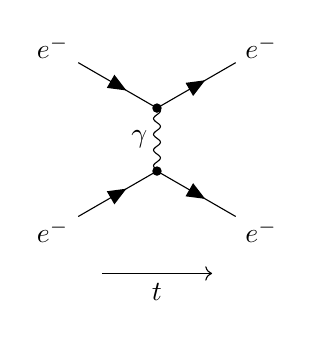
\begin{tikzpicture}
\begin{feynman}
\vertex (a);
\vertex [above=0.8cm of a] (b);
\vertex [below left=1.3cm and 0.7cm of a] (t1);
\vertex [below right=1.3cm and 0.7cm of a] (t2);
\vertex [below right=0.5cm and 1cm of a] (f1){$e^-$};
\vertex [below left=0.5cm and 1cm of a] (f2){$e^-$};
\vertex [above right=0.5cm and 1cm of b] (f3){$e^-$};
\vertex [above left=0.5cm and 1cm of b] (f4){$e^-$};
\diagram*{
(f2) -- [fermion] (a) -- [fermion] (f1),
(a) -- [boson, edge label=$\gamma$] (b),
(f4) -- [fermion] (b) -- [fermion] (f3),
};
\end{feynman}
\draw[->] (t1) -- (t2) node[midway, below] {$t$};
\fill (a) circle (0.06cm);
\fill (b) circle (0.06cm);
\end{tikzpicture}
\caption{t-Kanal}
\end{figure}\\
Für den Prozess $\gamma\gamma\longrightarrow \gamma\gamma$:
\begin{figure}[h!]
\centering
\begin{minipage}{0.3\textwidth}
\centering
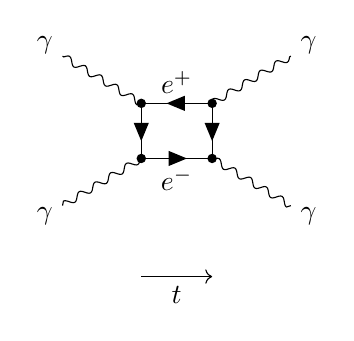
\begin{tikzpicture}
\begin{feynman}
\vertex (a);
\vertex [right=0.9cm of a] (b);
\vertex [above=0.7cm of a] (c);
\vertex [above=0.7cm of b] (d);
\vertex [below=of a] (t1);
\vertex [below=of b] (t2);
\vertex [above left=0.5cm and 1cm of c] (f1){$\gamma$};
\vertex [below left=0.5cm and 1cm of a] (f2){$\gamma$};
\vertex [above right=0.5cm and 1cm of d] (f3){$\gamma$};
\vertex [below right=0.5cm and 1cm of b] (f4){$\gamma$};
\diagram*{
(f1) -- [boson] (c) -- [fermion] (a) -- [boson] (f2),
(a) -- [fermion, edge label'=$e^-$] (b),
(d) -- [fermion, edge label'=$e^+$] (c),
(f3) -- [boson] (d) -- [fermion] (b) -- [boson] (f4),
};
\end{feynman}
\draw[->] (t1) -- (t2) node[midway, below] {$t$};
\fill (a) circle (0.06cm);
\fill (b) circle (0.06cm);
\fill (c) circle (0.06cm);
\fill (d) circle (0.06cm);
\end{tikzpicture}
\end{minipage}
\begin{minipage}{0.3\textwidth}
\centering
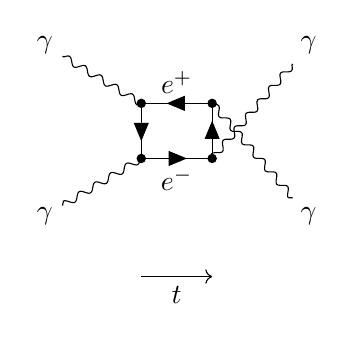
\begin{tikzpicture}
\begin{feynman}
\vertex (a);
\vertex [right=0.9cm of a] (b);
\vertex [above=0.7cm of a] (c);
\vertex [above=0.7cm of b] (d);
\vertex [below=of a] (t1);
\vertex [below=of b] (t2);
\vertex [above left=0.5cm and 1cm of c] (f1){$\gamma$};
\vertex [below left=0.5cm and 1cm of a] (f2){$\gamma$};
\vertex [above right=0.5cm and 1cm of d] (f3){$\gamma$};
\vertex [below right=0.5cm and 1cm of b] (f4){$\gamma$};
\diagram*{
(f1) -- [boson] (c),
(a) -- [boson] (f2),
(a) -- [fermion, edge label'=$e^-$] (b) -- [fermion] (d) -- [fermion, edge label'=$e^+$] (c) -- [fermion] (a),
(f3) -- [boson] (b), 
(d) -- [boson] (f4),
};
\end{feynman}
\draw[->] (t1) -- (t2) node[midway, below] {$t$};
\fill (a) circle (0.06cm);
\fill (b) circle (0.06cm);
\fill (c) circle (0.06cm);
\fill (d) circle (0.06cm);
\end{tikzpicture}
\end{minipage}
\begin{minipage}{0.3\textwidth}
\centering
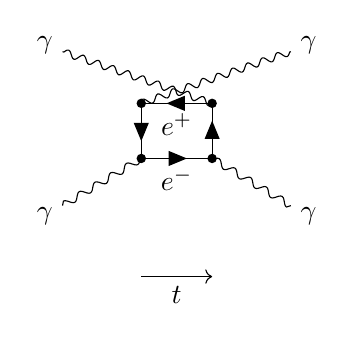
\begin{tikzpicture}
\begin{feynman}
\vertex (a);
\vertex [right=0.9cm of a] (b);
\vertex [above=0.7cm of a] (c);
\vertex [above=0.7cm of b] (d);
\vertex [below=of a] (t1);
\vertex [below=of b] (t2);
\vertex [above left=0.5cm and 1cm of c] (f1){$\gamma$};
\vertex [below left=0.5cm and 1cm of a] (f2){$\gamma$};
\vertex [above right=0.5cm and 1cm of d] (f3){$\gamma$};
\vertex [below right=0.5cm and 1cm of b] (f4){$\gamma$};
\diagram*{
(f1) -- [boson] (d),
(a) -- [boson] (f2),
(a) -- [fermion, edge label'=$e^-$] (b) -- [fermion] (d) -- [fermion, edge label=$e^+$] (c) -- [fermion] (a),
(f3) -- [boson] (c), 
(b) -- [boson] (f4),
};
\end{feynman}
\draw[->] (t1) -- (t2) node[midway, below] {$t$};
\fill (a) circle (0.06cm);
\fill (b) circle (0.06cm);
\fill (c) circle (0.06cm);
\fill (d) circle (0.06cm);
\end{tikzpicture}
\end{minipage}
\end{figure}\\
Für den Prozess $e^-\gamma\longrightarrow e^-\gamma$:
\begin{figure}[h!]
\centering
\begin{minipage}{0.4\textwidth}
\centering
\begin{tikzpicture}
\begin{feynman}
\vertex (a);
\vertex [right=of a] (b);
\vertex [below=of a] (t1);
\vertex [below=of b] (t2);
\vertex [above left=of a] (f1){$\gamma$};
\vertex [below left=of a] (f2){$e^-$};
\vertex [above right=of b] (f3){$\gamma$};
\vertex [below right=of b] (f4){$e^-$};
\diagram*{
(f2) -- [fermion] (a) -- [fermion, edge label=$e^-$] (b) -- [fermion] (f4),
(f1) -- [boson] (a),
(b) -- [boson] (f3),
};
\end{feynman}
\draw[->] (t1) -- (t2) node[midway, below] {$t$};
\fill (a) circle (0.06cm);
\fill (b) circle (0.06cm);
\end{tikzpicture}
\caption{s-Kanal}
\end{minipage}
\begin{minipage}{0.4\textwidth}
\centering
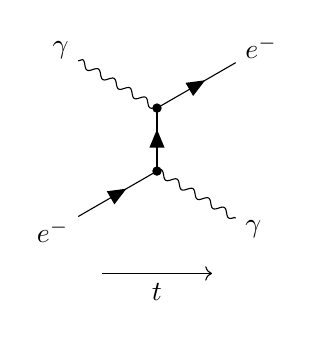
\begin{tikzpicture}
\begin{feynman}
\vertex (a);
\vertex [above=0.8cm of a] (b);
\vertex [below left=1.3cm and 0.7cm of a] (t1);
\vertex [below right=1.3cm and 0.7cm of a] (t2);
\vertex [below right=0.5cm and 1cm of a] (f1){$\gamma$};
\vertex [below left=0.5cm and 1cm of a] (f2){$e^-$};
\vertex [above right=0.5cm and 1cm of b] (f3){$e^-$};
\vertex [above left=0.5cm and 1cm of b] (f4){$\gamma$};
\diagram*{
(f2) -- [fermion] (a) -- [fermion] (b) -- [fermion] (f3),
(f1) -- [boson] (a),
(b) -- [boson] (f4),
};
\end{feynman}
\draw[->] (t1) -- (t2) node[midway, below] {$t$};
\fill (a) circle (0.06cm);
\fill (b) circle (0.06cm);
\end{tikzpicture}
\caption{t-Kanal}
\end{minipage}
\end{figure}\\
Für den Prozess $e^-e^+\longrightarrow\mu^-\mu^+$: 
\begin{figure}[h!]
\centering
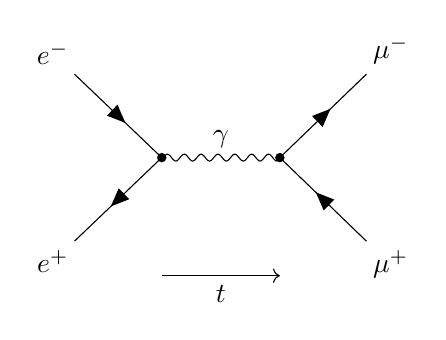
\begin{tikzpicture}
\begin{feynman}
\vertex (a);
\vertex [right=of a] (b);
\vertex [below=of a] (t1);
\vertex [below=of b] (t2);
\vertex [above left=of a] (f1){$e^-$};
\vertex [below left=of a] (f2){$e^+$};
\vertex [above right=of b] (f3){$\mu^-$};
\vertex [below right=of b] (f4){$\mu^+$};
\diagram*{
(f1) -- [fermion] (a) -- [fermion] (f2),
(a) -- [boson, edge label=$\gamma$] (b),
(f4) -- [fermion] (b) -- [fermion] (f3),
};
\end{feynman}
\draw[->] (t1) -- (t2) node[midway, below] {$t$};
\fill (a) circle (0.06cm);
\fill (b) circle (0.06cm);
\end{tikzpicture}
\caption{s-Kanal}
\end{figure}\,\newpage\,
Für den Prozess $e^-e^+\longrightarrow\gamma\gamma$:
\begin{figure}[h!]
\centering
\begin{minipage}{0.4\textwidth}
\centering
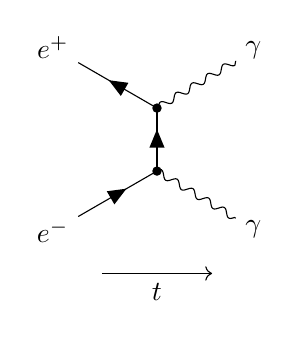
\begin{tikzpicture}
\begin{feynman}
\vertex (a);
\vertex [above=0.8cm of a] (b);
\vertex [below left=1.3cm and 0.7cm of a] (t1);
\vertex [below right=1.3cm and 0.7cm of a] (t2);
\vertex [below right=0.5cm and 1cm of a] (f1){$\gamma$};
\vertex [below left=0.5cm and 1cm of a] (f2){$e^-$};
\vertex [above right=0.5cm and 1cm of b] (f3){$\gamma$};
\vertex [above left=0.5cm and 1cm of b] (f4){$e^+$};
\diagram*{
(f2) -- [fermion] (a) -- [fermion] (b) -- [fermion] (f4),
(f1) -- [boson] (a),
(b) -- [boson] (f3),
};
\end{feynman}
\draw[->] (t1) -- (t2) node[midway, below] {$t$};
\fill (a) circle (0.06cm);
\fill (b) circle (0.06cm);
\end{tikzpicture}
\caption{t-Kanal}
\end{minipage}
\begin{minipage}{0.4\textwidth}
\centering
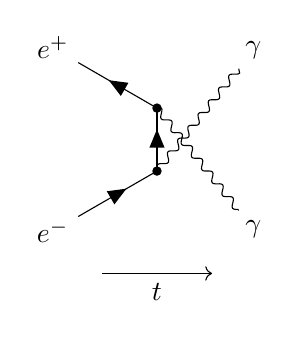
\begin{tikzpicture}
\begin{feynman}
\vertex (a);
\vertex [above=0.8cm of a] (b);
\vertex [below left=1.3cm and 0.7cm of a] (t1);
\vertex [below right=1.3cm and 0.7cm of a] (t2);
\vertex [below right=0.5cm and 1cm of a] (f1){$\gamma$};
\vertex [below left=0.5cm and 1cm of a] (f2){$e^-$};
\vertex [above right=0.5cm and 1cm of b] (f3){$\gamma$};
\vertex [above left=0.5cm and 1cm of b] (f4){$e^+$};
\diagram*{
(f2) -- [fermion] (a) -- [fermion] (b) -- [fermion] (f4),
(f1) -- [boson] (b),
(a) -- [boson] (f3),
};
\end{feynman}
\draw[->] (t1) -- (t2) node[midway, below] {$t$};
\fill (a) circle (0.06cm);
\fill (b) circle (0.06cm);
\end{tikzpicture}
\caption{t-Kanal}
\end{minipage}
\end{figure}\\
Für den Prozess $\gamma\gamma\longrightarrow e^-e^+$:
\begin{figure}[h!]
\centering
\begin{minipage}{0.4\textwidth}
\centering
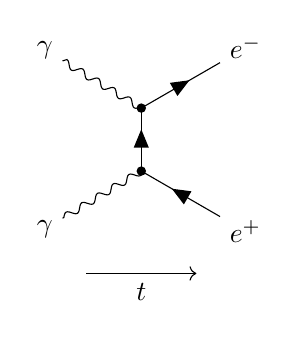
\begin{tikzpicture}
\begin{feynman}
\vertex (a);
\vertex [above=0.8cm of a] (b);
\vertex [below left=1.3cm and 0.7cm of a] (t1);
\vertex [below right=1.3cm and 0.7cm of a] (t2);
\vertex [below right=0.5cm and 1cm of a] (f2){$e^+$};
\vertex [below left=0.5cm and 1cm of a] (f1){$\gamma$};
\vertex [above right=0.5cm and 1cm of b] (f4){$e^-$};
\vertex [above left=0.5cm and 1cm of b] (f3){$\gamma$};
\diagram*{
(f2) -- [fermion] (a) -- [fermion] (b) -- [fermion] (f4),
(f1) -- [boson] (a),
(b) -- [boson] (f3),
};
\end{feynman}
\draw[->] (t1) -- (t2) node[midway, below] {$t$};
\fill (a) circle (0.06cm);
\fill (b) circle (0.06cm);
\end{tikzpicture}
\caption{t-Kanal}
\end{minipage}
\begin{minipage}{0.4\textwidth}
\centering
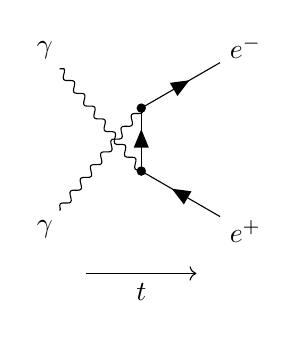
\begin{tikzpicture}
\begin{feynman}
\vertex (a);
\vertex [above=0.8cm of a] (b);
\vertex [below left=1.3cm and 0.7cm of a] (t1);
\vertex [below right=1.3cm and 0.7cm of a] (t2);
\vertex [below right=0.5cm and 1cm of a] (f2){$e^+$};
\vertex [below left=0.5cm and 1cm of a] (f1){$\gamma$};
\vertex [above right=0.5cm and 1cm of b] (f4){$e^-$};
\vertex [above left=0.5cm and 1cm of b] (f3){$\gamma$};
\diagram*{
(f2) -- [fermion] (a) -- [fermion] (b) -- [fermion] (f4),
(f1) -- [boson] (b),
(a) -- [boson] (f3),
};
\end{feynman}
\draw[->] (t1) -- (t2) node[midway, below] {$t$};
\fill (a) circle (0.06cm);
\fill (b) circle (0.06cm);
\end{tikzpicture}
\caption{t-Kanal}
\end{minipage}
\end{figure}
\end{document}